% Ovo je glavni fajl za generiranje predloska dokumenta doktorske disertacije Elektrotehnickog fakulteta u Sarajevu. 
% Verzija: 24. februar 2016. godine 

% Autor: Emir Sokic , esokic@etf.unsa.ba% 
% Bazirano na predlosku koji se koristi na FER Zagreb

%%%%%%%%%%%%%%%%%%%%%%%%%%%%%%%%%%%%%%%%%%%%%%%%%%%%%%%%%%%%%%%%%%%%%%
%%%%%%%%%%%%%%%%%%%%%%%%% POSTAVKE %%%%%%%%%%%%%%%%%%%%%%%%%%%%%%%%%%%
%%%%%%%%%%%%%%%%%%%%%%%%% NE MIJENJATI %%%%%%%%%%%%%%%%%%%%%%%%%%%%%%%
%%%%%%%%%%%%%%%%%%%%%%%%%%%%%%%%%%%%%%%%%%%%%%%%%%%%%%%%%%%%%%%%%%%%%%

\documentclass[12pt,oneside, a4paper]{book}

%Ovo su paketi koji se koriste za kompajliranje dokumenta
%Vecina paketa je ukljucena po defaultu u texlive 2013 i novijim verzijama
\usepackage{etex}
\usepackage{xcolor}
\usepackage[pdftex]{graphicx}
\usepackage{rotating}
\usepackage{epsfig}
\usepackage{epstopdf}
\usepackage[T1]{fontenc}
\usepackage[utf8]{inputenc}
\usepackage{cmap}
\usepackage[croatian]{babel}
\usepackage[unicode]{hyperref}
\usepackage{mathptmx}
\usepackage{amscd}
\usepackage{amssymb}
\usepackage{amsmath}
\usepackage{pdfpages}
\usepackage{amsfonts}
\usepackage[left=2.5cm,right=2.5cm,top=2.5cm,bottom=2.5cm]{geometry}
\usepackage{setspace} 
\usepackage{hhline}
\usepackage{enumerate}
\usepackage{delarray}
\usepackage{array}  
\usepackage{tabularx} 
\usepackage{multirow}  
\usepackage[bf, font=small]{caption}
\usepackage[labelfont=small, font=small]{subcaption}
\usepackage{wasysym}
\usepackage{subeqnarray}
\usepackage{pdflscape} % setting page into landscape view
\usepackage{enumitem} % for itemize lists
\usepackage[toc,page]{appendix}
\newcommand{\HRule}{\rule{\linewidth}{0.5mm}}
\usepackage{makeidx}
\usepackage{nomencl}
\usepackage{comment}
\usepackage{listings}
\lstset{basicstyle=\ttfamily,breaklines=true}
\usepackage{courier}
% Podesavanje izgleda zaglavlja i podnozja strana
\usepackage{fancyhdr}

\usepackage{multicol}

\fancypagestyle{plain}{%
  \fancyhf{}% Clear header/footer
  \fancyfoot[OR]{{\thepage}}%
  \fancyfoot[EL]{{\thepage}}%
  \renewcommand{\headrulewidth}{0pt}%
}

% required for printing index
% use \index{name} in text
%\usepackage{makeidx}
%\makeindex
% required for printing nomenclature
% use \nomenclature{symbol}{description} in text
%\usepackage{nomencl}
%\makenomenclature
%\renewcommand{\nomname}{Popis oznaka}




%Opcionalno
%\linespread{1.3}
%\setlist{nolistsep}   % setting for itemize lists
%\renewcommand{\thefootnote}{\fnsymbol{footnote}}  % to get unnumbered footnotes

% Adding a dot after chapter number in TOC 
%\let\savenumberline\numberline
%\def\numberline#1{\savenumberline{#1.}}



%\pagestyle{fancyplain}


%\rfoot{\thepage}
% iskljucivanje broja strane iz Sadrzaja, Popisa slika i Popisa tabela
\AtBeginDocument{\addtocontents{toc}{\protect\thispagestyle{empty}}}
\AtBeginDocument{\addtocontents{lof}{\protect\thispagestyle{empty}}}
\AtBeginDocument{\addtocontents{lot}{\protect\thispagestyle{empty}}}

%\rhead{\slshape \nouppercase \leftmark}
%\lhead{} %delete left header


%Podesavanje izgleda referenci
\usepackage[square, numbers, sort]{natbib} 

%Promjena naziva pojedinih poglavlja sa Hrvatskog na Bosanski
% Bibliography u "Literatura"
\addto\captionscroatian{%
  \renewcommand{\bibname}{Literatura}
  \renewcommand{\tablename}{Tabela}
  \renewcommand{\nomname}{Popis oznaka}
  \renewcommand{\indexname}{Indeks pojmova}
  \renewcommand{\lstlistingname}{Program}
}
%"Popis tablica" u "Popis tabela"
\addto\captionscroatian{\renewcommand{\listtablename}{Popis tabela}}
\addto\captionscroatian{\renewcommand\appendixname{Prilog}}
\addto\captionscroatian{\renewcommand\appendixpagename{Prilozi}}
\renewcommand\appendixtocname{Prilozi}

\makeindex
\makenomenclature

%\usepackage{etoolbox}
%\patchcmd{\chapter}{\thispagestyle{plain}}{\thispagestyle{fancyplain}}{}{}


\begin{document}

%%%%%%%%%%%%%%%%%%%%%%%%%%%%%%%%%%%%%%%%%%%%%%%%%%%%%%%%%%%%%%%%%%%%%%
%%%%%%%%%%%%%%%%%%%%%%%%% OSNOVNI DOKUMENT %%%%%%%%%%%%%%%%%%%%%%%%%%%
%%%%%%%%%%%%%%%%%%%%%%%%%%%%%%%%%%%%%%%%%%%%%%%%%%%%%%%%%%%%%%%%%%%%%%

\frontmatter

%%%%%%%%%%%%%%%%%%%% NASLOVNA STRANA %%%%%%%%%%%%%%%%%%%%%%%%
\begin{titlepage}
\begin{center}


\includegraphics[width=0.25\textwidth]{etf-logo.png}~\\[0.1cm]
\textsc{\Large Univerzitet u Sarajevu}\\[0.2cm]  
\textsc{\Large Elektrotehnički fakultet}\\[0.2cm] 
\textsc{\Large Odsjek za automatiku i elektroniku}\\[3cm]\HRule \\[0.5cm] 
{\huge \bfseries Upravljanje električnim vozilom} \\[0.4cm] 
\HRule \\[0.5cm]

\textsc{\Large Projektni zadatak}\\[0.4cm]
\textsc{\Large - Drugi ciklus studija - }\\[1.5cm]

% Author and supervisor 
\textbf{ 
\Large Student:\\  
\Large Vedad Halimić\\[1cm]  
\Large Mentor: \\[0.2cm] 
\Large V. prof. dr Senad Huseinbegović.} 
\vfill

% Bottom of the page  
{\large Sarajevo, novembar 2021.}

\end{center} 
\end{titlepage}

% Sažetak (na Bosanskom jeziku i na Engleskom jeziku),
% postavka rada i izjava o autentičnoati su dati kao odvojeni fajlovi


%%%%%%%%%%%%%% SAŽETAK I ABSTRACT %%%%%%%%%%%%%%%%%%%%%%%%%%%%%%%
%\include{abstract}

%%%%%%%%%%%%%%%%%%%% POSTAVKA RADA %%%%%%%%%%%%%%%%%%%%%%%%%%%%%%%
%\include{postavka}

%%%%%%%%%%%%%%%%%%%% POTPISI CLANOVA KOMISIJE %%%%%%%%%%%%%%%%%%%%
% uključiti po potrebi
%\include{potpisi}

%%%%%%%%%%%%%%%%%%%% PREDGOVOR %%%%%%%%%%%%%%%%%%%%
% uključiti po želji autora
%\include{predgovor}

%%%%%%%%%%%%%%%%%%%% IZJAVA AUTORA %%%%%%%%%%%%%%%%%%%%
%\include{izjava}

%%%%%%%%%%%%%%% SADRŽAJ %%%%%%%%%%%%%%%%%%%%%%%
%\clearpage
\tableofcontents

%%%%%%%%%%%%%%% POPIS SLIKA %%%%%%%%%%%%%%%%%%%%%%%%%%%
%\clearpage
%\listoffigures
%\addcontentsline{toc}{chapter}{Popis slika}

%%%%%%%%%%%%%%% POPIS TABELA %%%%%%%%%%%%%%%%%%%%%%%%%%
%\clearpage
%\listoftables
%\addcontentsline{toc}{chapter}{Popis tabela}

%%%%%%%%%%%%%%% POPIS OZNAKA %%%%%%%%%%%%%%%%%%%%%%%%%%%
%\clearpage
%\printnomenclature
%\addcontentsline{toc}{chapter}{Popis oznaka}


\cleardoublepage % start new page
\pagestyle{fancyplain} % puts headers/footers back on
\fancyhf{}
\lhead{\nouppercase{\fancyplain{}{\leftmark}}}
\renewcommand{\chaptermark}[1]{\markboth{#1}{}}
\renewcommand{\footrulewidth}{0.4pt} %draw foot line
\lfoot{\slshape Halimić, V., Projektni zadatak}
\rfoot{\thepage}
\cfoot{}

%%%%%%%%%%%%%%%%%%%%%%%%%%%%%%%%%%%%%%%%%%%%%%%%%%%%%%%%%%%%%%%%%%%%%%
\mainmatter


%%%%%%%%%%%%%%%%%%%%%%%%%%%%%%%%%%%%%%%%%%%%%%%%%%%%%%%%%%%%%%%%%%%%%%
%%%%%%%%%%%%%%%%%%%%%%%%% POGLAVLJA %%%%%%%%%%%%%%%%%%%%%%%%%%%%%%%%%%
%%%%%%%%%%%%%%%%%%%%%%%%%%%%%%%%%%%%%%%%%%%%%%%%%%%%%%%%%%%%%%%%%%%%%%
%Poglavlja je najbolje raditi u odvojenim fajlovima
%Poglavlje 1
%\include{poglavlje_1}
%Poglavlje 2
%\include{poglavlje_2}
%Poglavlje 3
%\include{poglavlje_3}

\chapter{Uvod}

\qquad U ovom radu je predstavljeno upravljanje električnim vozilom (slika \ref{fig:buggy}) sa pogonom na sva četiri točka. Proizvođač \href{https://www.qsmotor.com/product/8000w-car-motor/}{motora} je kompanija \textit{QSMOTOR}. Snaga motora je $8000W$, a standardni napon napajanja iznosi $72V$. Svaki od motora je spojen na odgovarajući pretvarač/\href{https://kellycontroller.com/shop/kls-h/}{invertor}. Motori su trofazni i sadrže dva seta Hallovih senzora za određivanje brzine i pozicije. Datasheet motora je dat u prilogu \ref{motor_datasheet}, a dio dokumentacije pretvarača \textit{KLS7275H} u prilogu \ref{kelly_datasheet}. Razvoj upravljačkog prototipa će biti realiziran pomoću \href{https://www.dspace.com/en/inc/home/products/hw/microlabbox.cfm?fbclid=IwAR08_hHwsXPVRs6ng2DLSU5HA3vDNzpBa9CMpO8DWlSQ1DXPK58BkLmoiRE}{dSpace} sistema.

\begin{figure}
\begin{center}
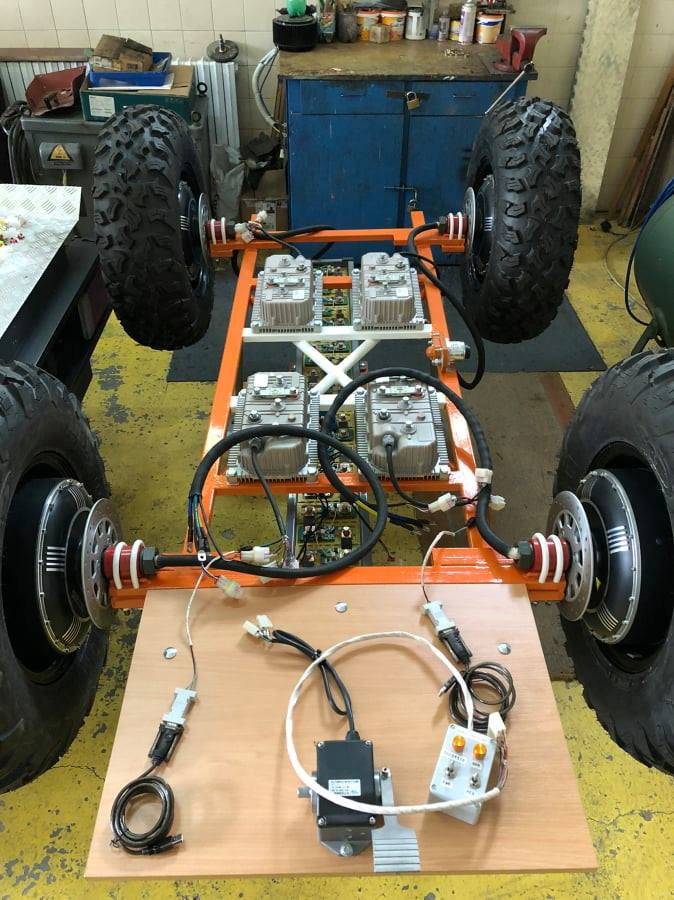
\includegraphics[scale=0.5]{slike/electric_car.jpg}
\end{center}
\caption{Električno $4x4$ vozilo}
\label{fig:buggy}
\end{figure}

\section{Motor}

\qquad Motor je trofazni sa $16$ pari polova, nominalne snage $8000W$. Za mjerenje brzine i pozicije motora, dostupna su dva seta Hallovih senzora. Moguće je mjeriti i temperaturu motora pomoću temperaturnog senzora $KTY83/122$. Motor sadrži dva konektora, čiji pinovi odgovaraju pinovima na \textit{DJ7061Y-2.3-21} konektoru energetskog pretvarača. Svaki od konektora daje informacije sa Hallovog i temperaturnog senzora.

\section{Pretvarač}

\qquad Energetski pretvarač \textit{KLS7275H} proizvođača \textit{Kelly} sadrži 5 digitalnih ulaza: prekidače za gas i kočnicu, prekidače za kretanje naprijed i nazad, te prekidač za \textit{boost} način rada. Dostupna su 3 analogna ulaza: gas, kočnica i temperatura motora. Opseg ulaznog napona može varirati od $0$ do $5V$. Za upravljanje je moguće koristiti i palicu (\textit{engl. joystick}), pri čemu pozicija palice određuje zadanu brzinu i smjer kretanja. \textit{Cruise} režim rada, koji je također dostupan, podrazumijeva zadržavanje zadane brzine vrtnje motora sve dok se ne zada nova brzina ili aktivira kočnica. Pretvarač podržava povezivanje putem \textit{CAN} mreže.

\subsection{Pinovi energetskog pretvarača}

\qquad \textit{KLS7275H} kontroler posjeduje tri konektora prikazana na slici (\ref{fig:kellypins} i 22 pina. Pored standardnih pinova za napajanje, pretvarač posjeduje pinove za prikupljanje informacija sa motora (Hallov senzor i temperaturni senzor), kao i pinove za definiranje smjera i brzine vrtnje motora. Žica spojena na odgovarajući pin je označena jedinstvenom bojom i brojem. Funkcije pinova su date u nastavku.

\begin{itemize}
	\item Konektor \textit{DJ7091Y-2.3-11}
	\begin{itemize}
		\item REV-SW (14) - prekidač za kretanje nazad
		\item GND (6) - minus napona napajanja, povratni signal
		\item FWD (12) - prekidač za kretanje naprijed
		\item 12V (11) - naponski izvor od $12V$
		\item 12V Brake (25) - ručna kočnica
		\item ECO (22) - prekidač za štedljivi način rada
		\item CAN-H (33) - \textit{high} pin za CAN komunikaciju
		\item PWR (7) - plus napona napajanja pretvarača
		\item CAN-L (34) - \textit{low} pin za CAN komunikaciju
	\end{itemize}
	\item Konektor \textit{DJ7091Y-2.3-21}
		\begin{itemize}
		\item FOOT-SW (15) - prekidač za gas
		\item Throttle (3) - analogni ulaz za gas ($0-5V$)
		\item GND (20) - minus napon napajanja, povratni signal
		\item Meter (8) - kopija signala sa Hallovog senzora
		\item 5V (4) - naponski izvor od $5V$
		\item Brake-AN (2) - \textit{boost} funkcija ili analogni ulaz za regenerativni tip kočenja
		\item 12V (11) - naponski izvor od $12V$
	\end{itemize}
	\item Konektor \textit{DJ7061Y-2.3-21}
		\begin{itemize}
		\item GND (21) - minus napon napajanja, povratni signal
		\item Temp (1) - temperatura motora
		\item 5V (5) - naponski izvor od $5V$
		\item Hall A (18) - signal Hallovog senzora za fazu A
		\item Hall B (17) - signal Hallovog senzora za fazu B 
		\item Hall C (16) - signal Hallovog senzora za fazu C 
	\end{itemize}
\end{itemize}

\begin{figure}
\begin{center}
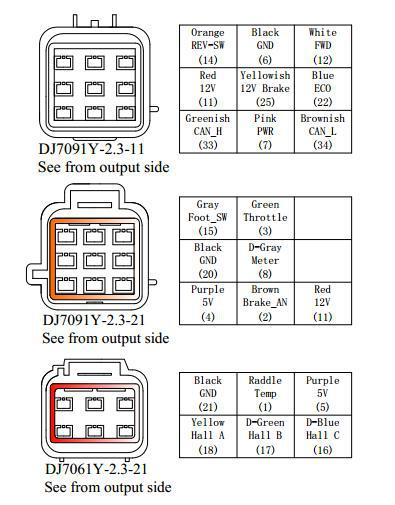
\includegraphics[scale=1]{slike/kellypins.jpg}
\end{center}
\caption{Pinovi \textit{Kelly KLS7275H} pretvarača}
\label{fig:kellypins}
\end{figure}

\section{Upravljanje motorom}

\qquad Energetski pretvarač/kontroler koristi vektorsku modulaciju (\textit{engl. space-vector modulation}) za upravljanje trofaznim motorom. Za upravljanje cjelokupnim sistemom vozila, potrebno je uključiti dodatni sloj upravljanja, koji će upravljati paralelno sa sva četiri motora.

\section{Papučica gasa}

\qquad Brzinu motora je moguće zadavati pomoću papučice gasa. Model koji je odabran ima serijski broj \textit{JKH-005-A-65}. Prema specifikaciji proizvođača \textit{SAYOO}, datoj u prilogu \ref{gas}, dužina kabla spojenog na kočnicu iznosi $65cm$. U kablu se nalazi 5 žica raspoređenih na dva konektora - jedan sa tri, drugi sa četiri žice. Raspon ulaznog i izlaznog napona papučice gasa iznosi od $0$ do $5V$. Ovaj element se konceptualno ponaša kao otpornik sa klizačem koji je spojen na napon napajanja. Izlazni napon otpornika ovisi o položaju klizača, odnosno u ovom slučaju - položaja papučice gasa. Pinovi, prikazani na slici (\ref{fig:gas}), imaju funkcije date u nastavku.

\begin{itemize}
	\item (1) - plus napon napajanja ($5V$)
	\item (2) - minus napon napajanja ($0V$, masa)
	\item (3) - izlazni napon
	\item (4) - izlaz prekidača
	\item (5) - ulaz prekidača
\end{itemize}

\begin{figure}
\centering
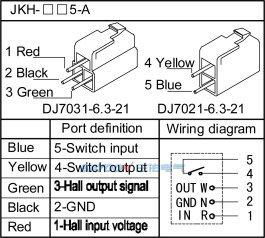
\includegraphics[scale=1]{slike/foot_throttle.png}
\caption{Pinovi papučice gasa}
\label{fig:gas}
\end{figure}









%%%%%%%%%%%%%%%%%%%%%%%%%%%%%%%%%%%%%%%%%%%%%%%%%%%%%%%%%%%%%%%%%%%%%%
%%%%%%%%%%%%%%%%%%%%%%%%% PRILOZI %%%%%%%%%%%%%%%%%%%%%%%%%%%%%%%%%%%%
%%%%%%%%%%%%%%%%%%%%%%%%%%%%%%%%%%%%%%%%%%%%%%%%%%%%%%%%%%%%%%%%%%%%%%
\begin{appendices}
%Priloge je najbolje raditi u odvojenim fajlovima
%Prilog 1
\chapter{Instalacija dSPACE programa}\label{dSpace}

\qquad Za razvoj upravljačkog algoritma korištenjem \textit{MicroLabBox} razvojnog sistema je potrebno instalirati \textit{dSPACE} softver koji će se integrirati sa \textit{Matlab/Simulink} okruženjem. U nastavku će biti dat proces instalacije \textit{dSPACE} programskog paketa, verzije \textbf{2018-A}.

\section{Tekstualni i video vodič za instalaciju}

\qquad Na zvaničnoj stranici proizvođača je moguće pronaći tekstualne (\textit{.pdf}) \cite{dSPACEinstall} i video \cite{dSPACEvideo} instrukcije za instalaciju \textit{dSPACE} softvera.

\section{Datoteke za instalaciju softvera}\label{folder}

\qquad Uz \textit{MicroLabBox} razvojni sistem dolaze dva DVD-a, na kojima se nalaze datoteke potrebne za instalaciju softvera. Detaljna uputstva za instalaciju se nalaze u datoteci \textbf{InstallingdSPACESoftware.pdf}. 

Vlasnici dSPACE licence i registrirani korisnici softver mogu preuzeti preko \href{https://www.dspace.com/en/pub/home/support/patches/rlsdl.cfm}{linka} koji vodi do zvanične internet stranice proizvođača. Pogodan način za instalaciju podrazumijeva kopiranje sadržaja sa oba DVD-a u isti folder na računaru, pri čemu je potrebno izvršiti prepisivanje (\textit{engl. overwrite}) odgovarajućih datoteka.

\section{Kompatibilne Matlab/Simulink distribucije}

\qquad dSPACE verzije 2018-A sadrži sljedeće programske komponente sa pripadajućim verzijama:

\begin{enumerate}
	\item RCP and HIL Software,
	\item AutomationDesk 5.6,
	\item TargetLink 4.3,
	\item Model Compare 2.8,
	\item dSPACE Python Extensions 2.5 i
	\item XIL API .NET MAPort 2018-A.
\end{enumerate}

Sve navedene komponente su kompatibilne sa \textit{Matlab} distribucijama \textbf{R2016b}, \textbf{R2017a} i \textbf{R2017b}. Djelimična kompatibilnost sa gorenavedenim programima se ostvaruje kroz distribucije R2016a (podržane stavke 3 i 4) i R2018a (podržane stavke: 1, 2, 5 i 6).

\section{Dodatne postavke}

\qquad Prije pokretanja instalacije \textit{dSPACE} softvera, potrebno je isključiti antivirusnu zaštitu i vatrozid (\textit{engl. firewall}) na računaru, kao i obezbjediti putem opcija za štednju energije (\textit{engl. power saving options}) da se računar neće isključiti ili preći u režim mirovanja (\textit{engl. sleep mode}) tokom procesa instalacije.

Također, potrebno je instalirati \textbf{MATLAB Support for MinGW-w64 C/C++ Compiler}, koji je moguće pronaći u \textit{Get Add-Ons} sekciji \textit{Matlabovog} korisničkog sučelja i \textbf{.NET Framework 3.5}.

\section{Proces instalacije dSPACE softvera}

\qquad Prije same instalacije je potrebno zatvoriti sve pokrenute programe. Kao što je navedeno u sekciji \ref{folder}, sadržaj sa oba DVD-a je pogodno kopirati u isti folder na računaru na koji se planira instalirati dSPACE i sa te lokacije \textbf{pokrenuti} instalaciju.

\subsection{Pokretanje instalacije}\label{pokretanje.instalacije}

\qquad Proces instalacije se započinje pokretanjem \textbf{Install\_Release.exe} datoteke. Pojavljuje se dijaloški okvir, prikazan na slici (\ref{fig:welcome}).

\begin{figure}[h]
\begin{center}
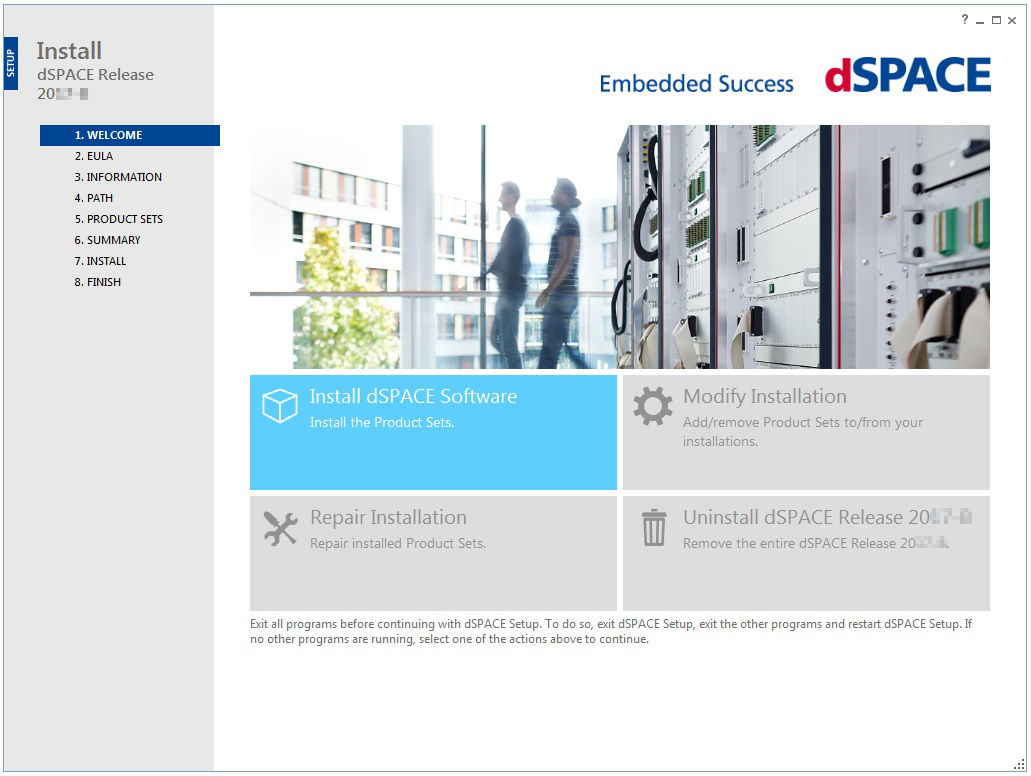
\includegraphics[width=\textwidth]{slike/dSpace/welcome.png}
\end{center}
\caption{Dijaloški okvir koji se pojavljuje nakon pokretanja instalacije \cite{dSPACEinstall}}
\label{fig:welcome}
\end{figure}

\textit{Napomena: \textit{dSPACE} od korisnika može tražiti ponovno pokretanje računara prije početka instalacije. Tada je potrebno \textit{restartovati} računar i vratiti se na korak \ref{pokretanje.instalacije}.}

\subsection{Instalacija, modifikacija, brisanje i popravljanje dSPACE softvera}

\qquad Dostupne opcije u dijaloškom okviru, koji je prikazan na slici \ref{fig:welcome}, mogu biti različite u zavisnosti od toga da li je na računaru već instaliran \textit{dSPACE} softver. Moguće opcije su:

\begin{itemize}
	\item Install \textit{dSPACE} Software - instalacija programa
	\item Modify Installation - dodavanje/brisanje dijelova programa iz već postojeće instalacije
	\item Repair Installation - popravljanje dijelova programa
	\item Uninstall \textit{dSPACE} Release 20$xx-x$ - brisanje svih instaliranih dijelova programa
\end{itemize}

Ukoliko na računaru nije već instaliran \textit{dSPACE}, jedina opcija koju je potrebno i moguće odabrati je \textbf{Install dSPACE Software}.

Nakon toga je potrebno \textbf{specificirati lokaciju} na kojoj će se instalirati \textit{dSPACE}. Pojavljuje se prozor prikazan na slici (\ref{fig:product.sets}).

\begin{figure}[h]
\begin{center}
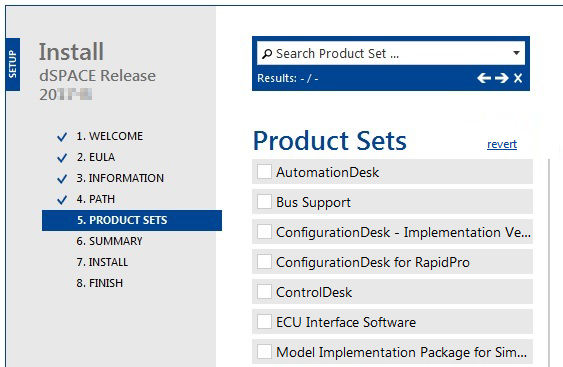
\includegraphics[width=\textwidth]{slike/dSpace/product sets.png}
\end{center}
\caption{Izbor dijelova programa za instalaciju \citep{dSPACEinstall}}
\label{fig:product.sets}
\end{figure}

\subsection{Instalacija dijelova programa}

\qquad U dijaloškom okviru, prikazanom na slici (\ref{fig:product.sets}), moguće je odabrati koji će se \textit{dSPACE} programski paketi instalirati na računar. Nakon što korisnik odabere željene pakete, potrebno je kliknuti na dugme \textbf{Next} u istom prozoru.

\subsection{Summary page}

\qquad Otvara se \textit{Summary page}, gdje je moguće odabrati sljedeće opcije:

\begin{itemize}
	\item Shut down after installation - Isključivanje računara nakon instalacije
	\item Start Installation Manager after installation - Pokretanje \textit{Installation Manager} programa nakon instalacije
\end{itemize}

Odabrati željene opcije i kliknuti na dugme \textbf{Start}.

\subsection{Završetak instalacije}

\qquad Potrebno je da korisnik izvrši ponovno pokretanje računara, kada to od njega instalacioni program bude tražio.

\subsection{Preuzimanje i instaliranje zakrpa}

\qquad Eventualne greške u instaliranom softveru se ispravljaju odgovarajućim zakrpama (\textit{engl. patches}) i ažuriranjima (\textit{engl. updates}). Na zvaničnoj stranici proizvođača \citep{dSPACEpatch} je moguće pronaći listu svih zakrpi i ažuriranja za odgovarajuću verziju \textit{dSPACE} softvera. Potrebno je \textbf{preuzeti} i \textbf{instalirati} date zakrpe.

\textit{Napomena: Pojedina ažuriranja i zakrpe zahtijevaju validni \textit{Software Maintenance Service} za preuzimanje i instalaciju.}

\section{Integracija dSPACE softvera sa Matlab/Simulink razvojnim okruženjem}

\qquad Instalirani \textit{dSPACE} softver je potrebno integrirati i povezati sa \textit{Matlab/Simulink} programskim paketom. To je moguće učiniti pomoću programa \textbf{dSPACE Installation Manager}.

Pokretanjem istog i navigacijom do \textbf{MATLAB} kartice (\textit{engl. tab}), dolazi se do prozora na kojem su prikazane sve \textit{Matlab} distribucije instalirane na računaru. \textit{dSPACE} je integriran sa odgovarajućom \textit{Matlab} distribucijom ukoliko se pored oznake \textbf{dSPACE Software Integration} nalazi \textit{integrated}, kao na slici (\ref{fig:matlab-integrate}).

\begin{figure}[h]
\begin{center}
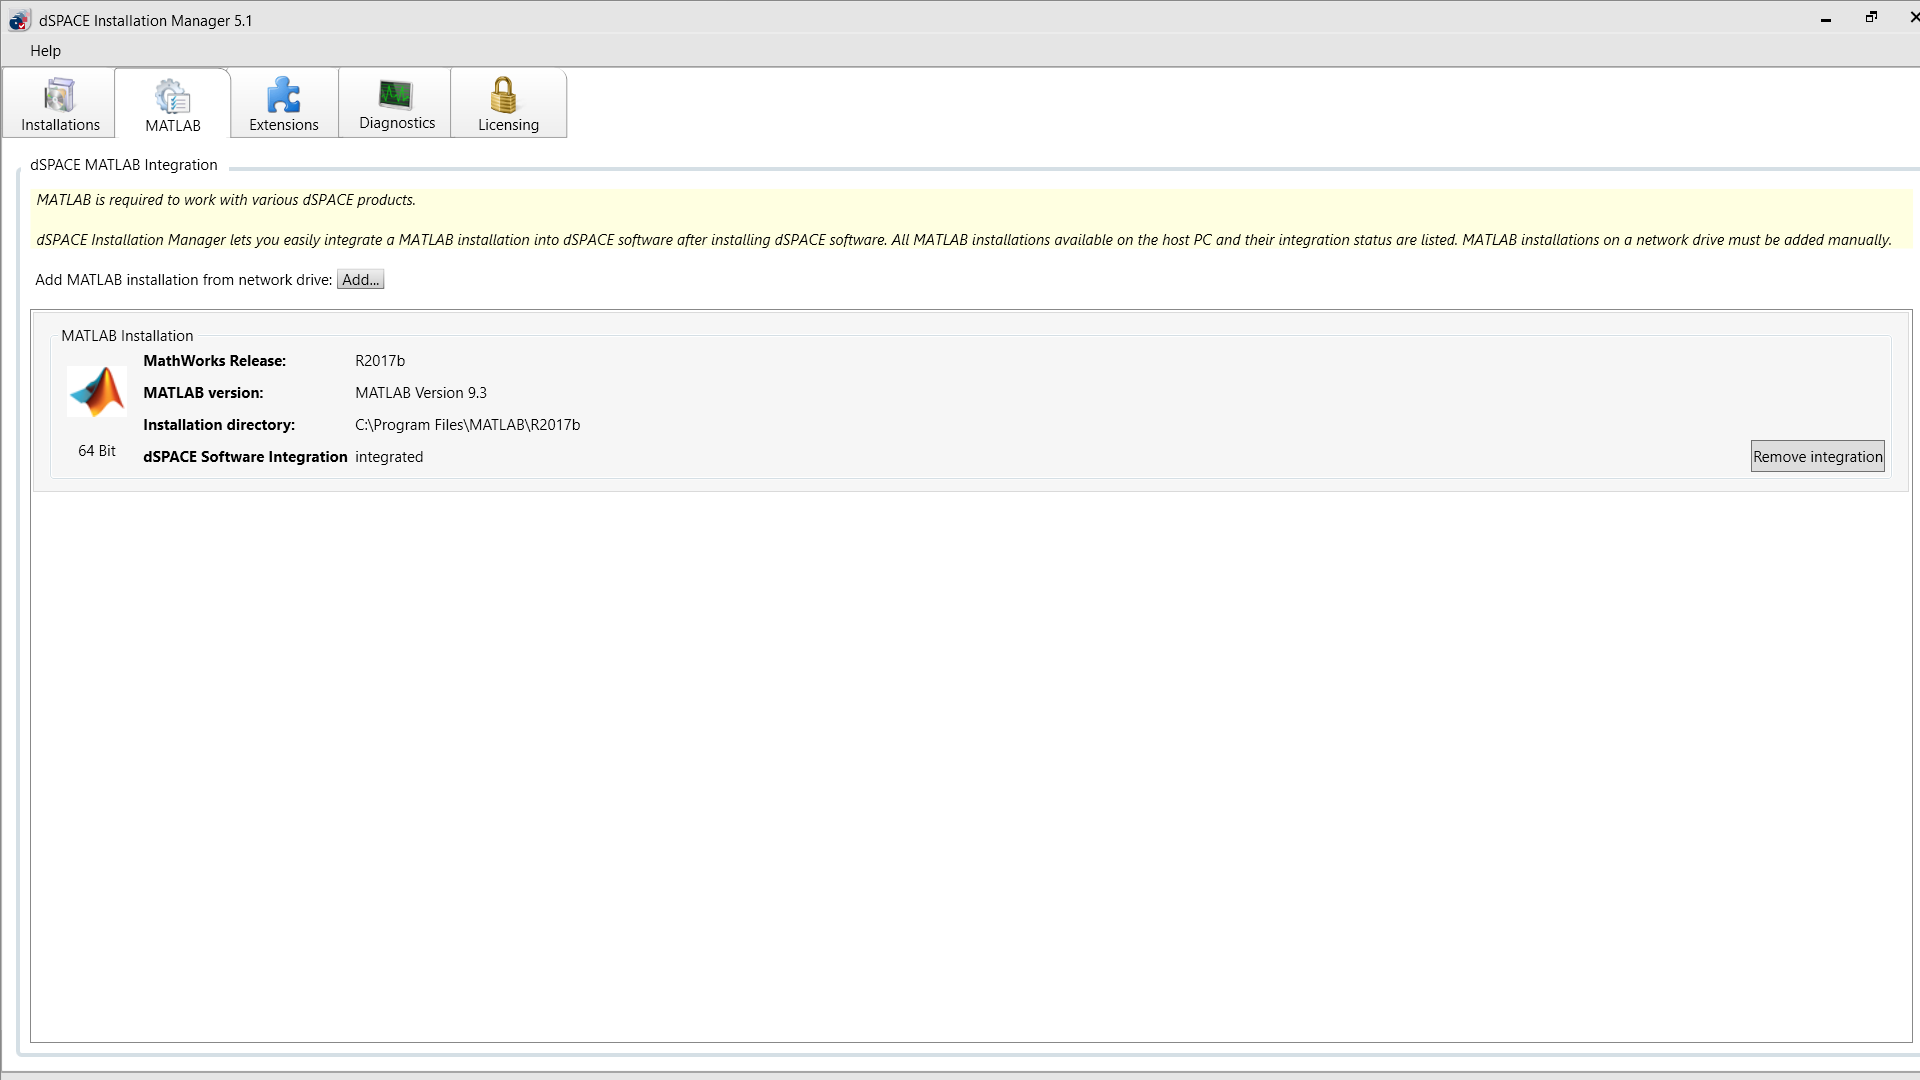
\includegraphics[width=\textwidth]{slike/dSpace/matlab-integrate.png}
\end{center}
\caption{Integracija \textit{dSPACE} instalacije sa odgovarajućom \textit{Matlab} distribucijom}
\label{fig:matlab-integrate}
\end{figure}

Pored integracije, potrebno je povezati (\textit{engl. connect}) dSPACE instalaciju sa odgovarajućom \textit{Matlab} distribucijom. U \textbf{dSPACE Installation Manager} programu je potrebno kroz \textit{Installations} i \textit{Installation Overview} kartice za svaku programsku komponentu, kod koje je dostupna ta opcija, u kartici \textit{Connect to MATLAB Release} - označiti (\textit{engl. check}) \textit{Connected} za odgovarajuću Matlab distribuciju, kao na slici (\ref{fig:matlab-connect}).

\begin{figure}[h]
\begin{center}
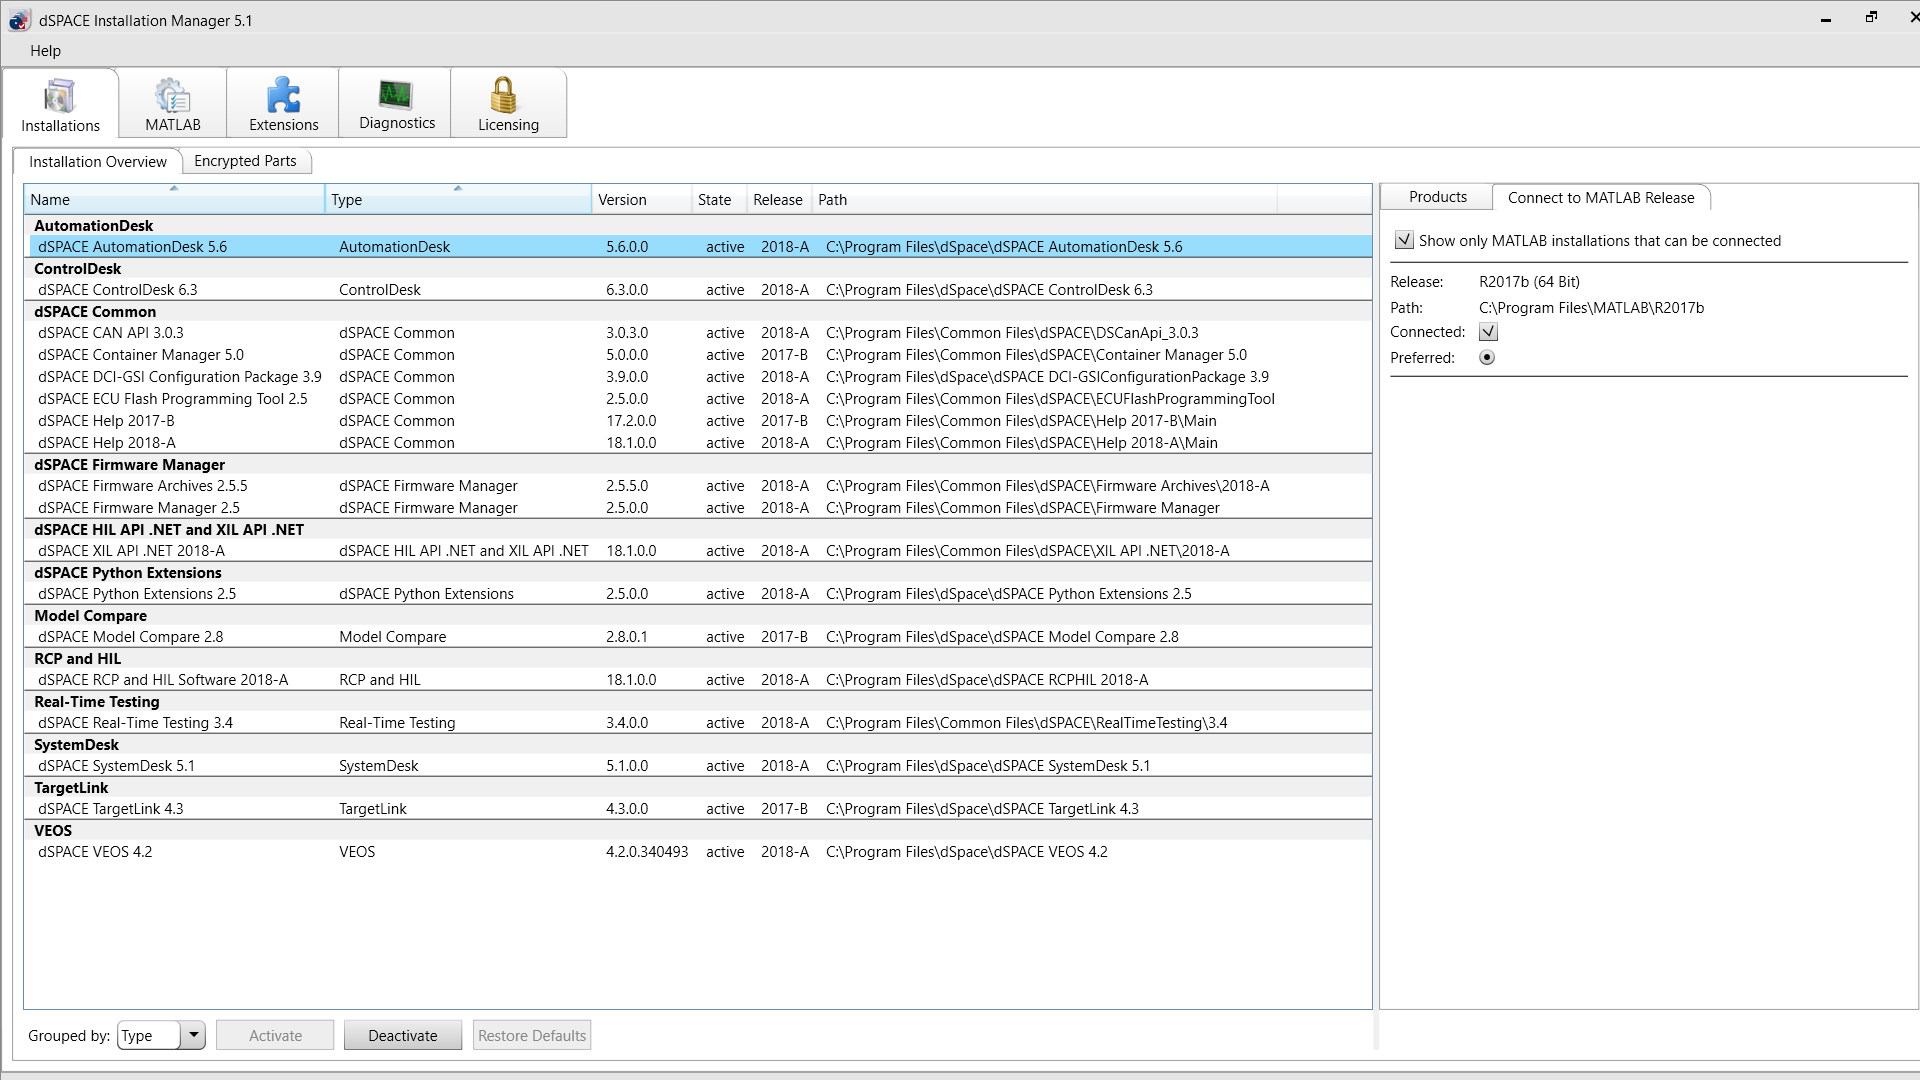
\includegraphics[width=\textwidth]{slike/dSpace/matlab-connect.png}
\end{center}
\caption{Povezivanje \textit{dSPACE} instalacije sa odgovarajućom \textit{Matlab} distribucijom}
\label{fig:matlab-connect}
\end{figure}

Prije pokretanja \textit{Matlab} distribucije, potrebno je zatvoriti dSPACE Installation Manager program sa ranije navedenom konfiguracijom. Programski paket \textit{Matlab} će pri pokretanju izvršiti \textit{konfiguraciju} dSPACE softvera, kao što je prikazano na slici (\ref{fig:matlab-configure}).

\begin{figure}[h]
\begin{center}
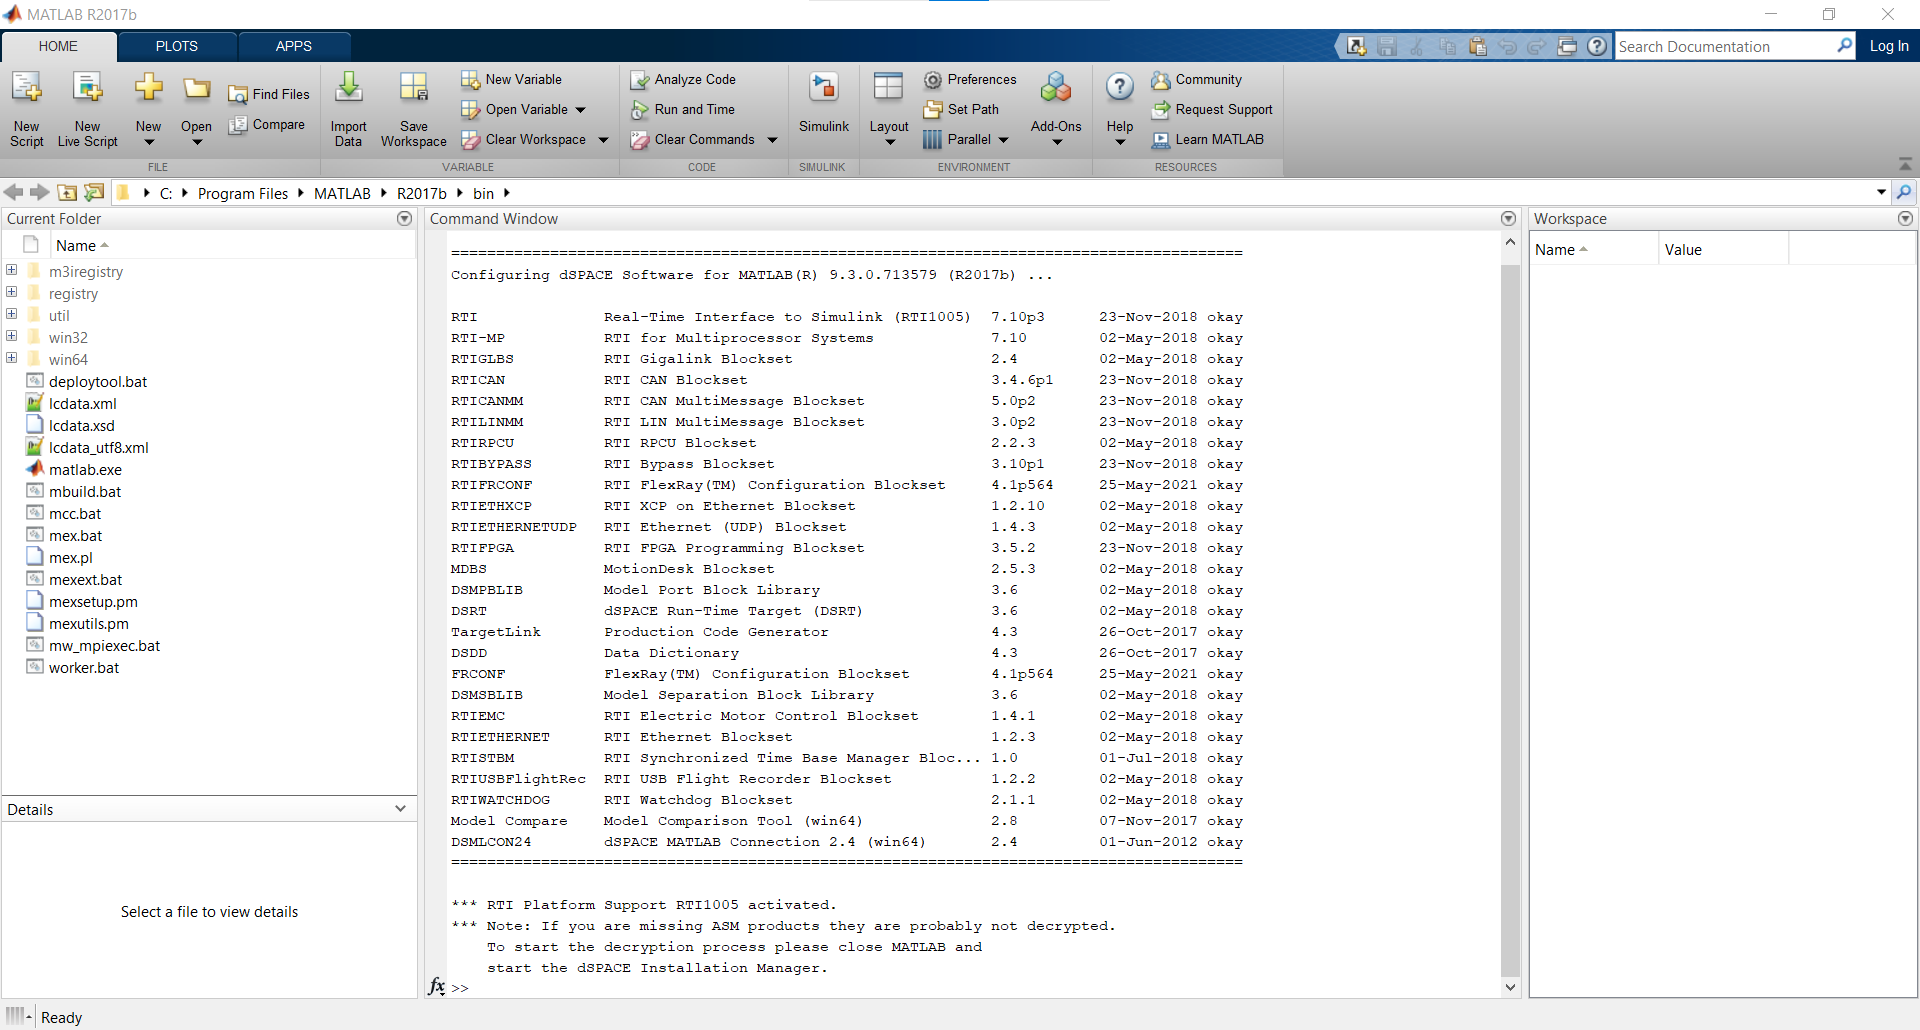
\includegraphics[width=\textwidth]{slike/dSpace/matlab-configure.png}
\end{center}
\caption{Konfiguracija \textit{dSPACE} softvera prilikom pokretanja Matlab distribucije}
\label{fig:matlab-configure}
\end{figure}

\section{Licenciranje i dekripcija dSPACE softvera}
\chapter{8000W DC Brushless Car Motor Datasheet}\label{motor_datasheet}

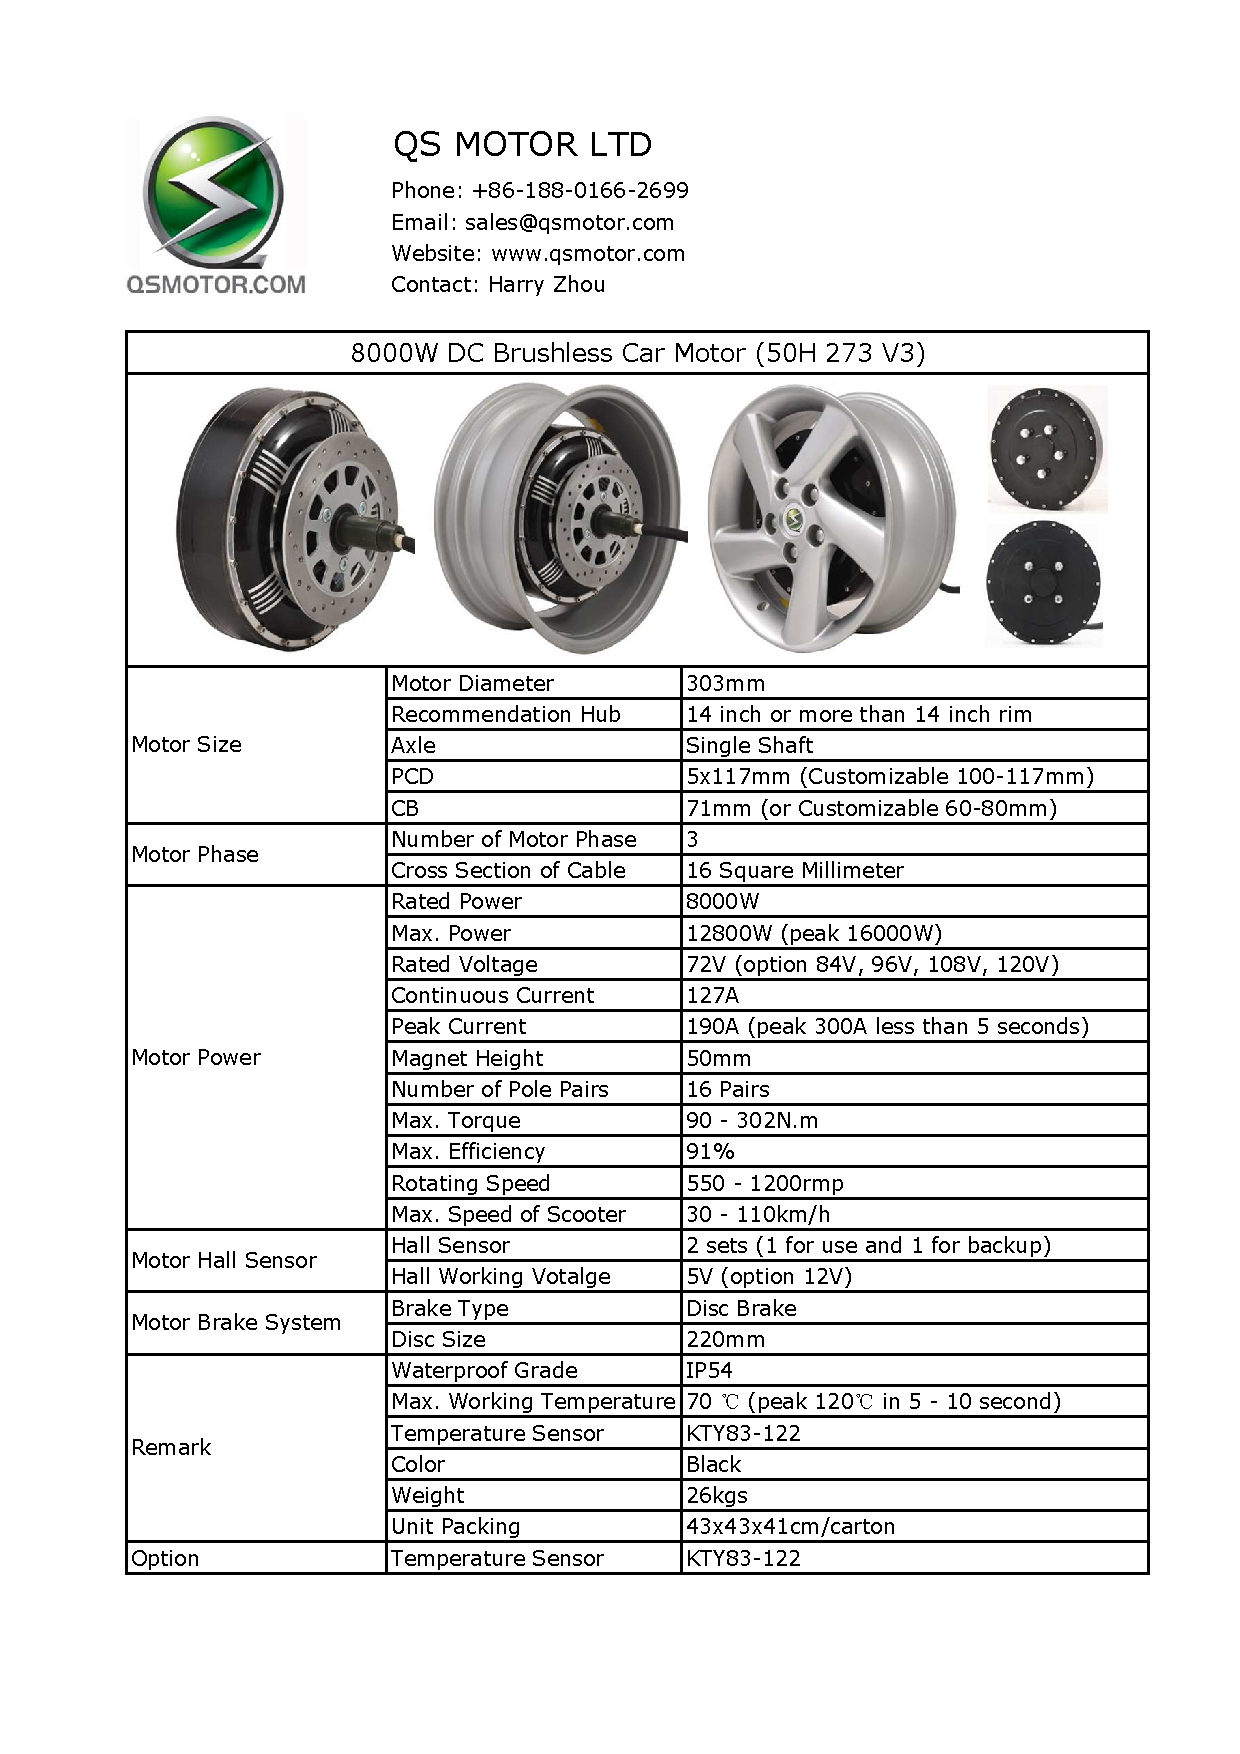
\includepdf[pages=-]{dokumenti/8000W Car Motor 72V}



%\chapter{Kelly KLS-H Brushless Motor Controller User's Manual}\label{kelly_datasheet}

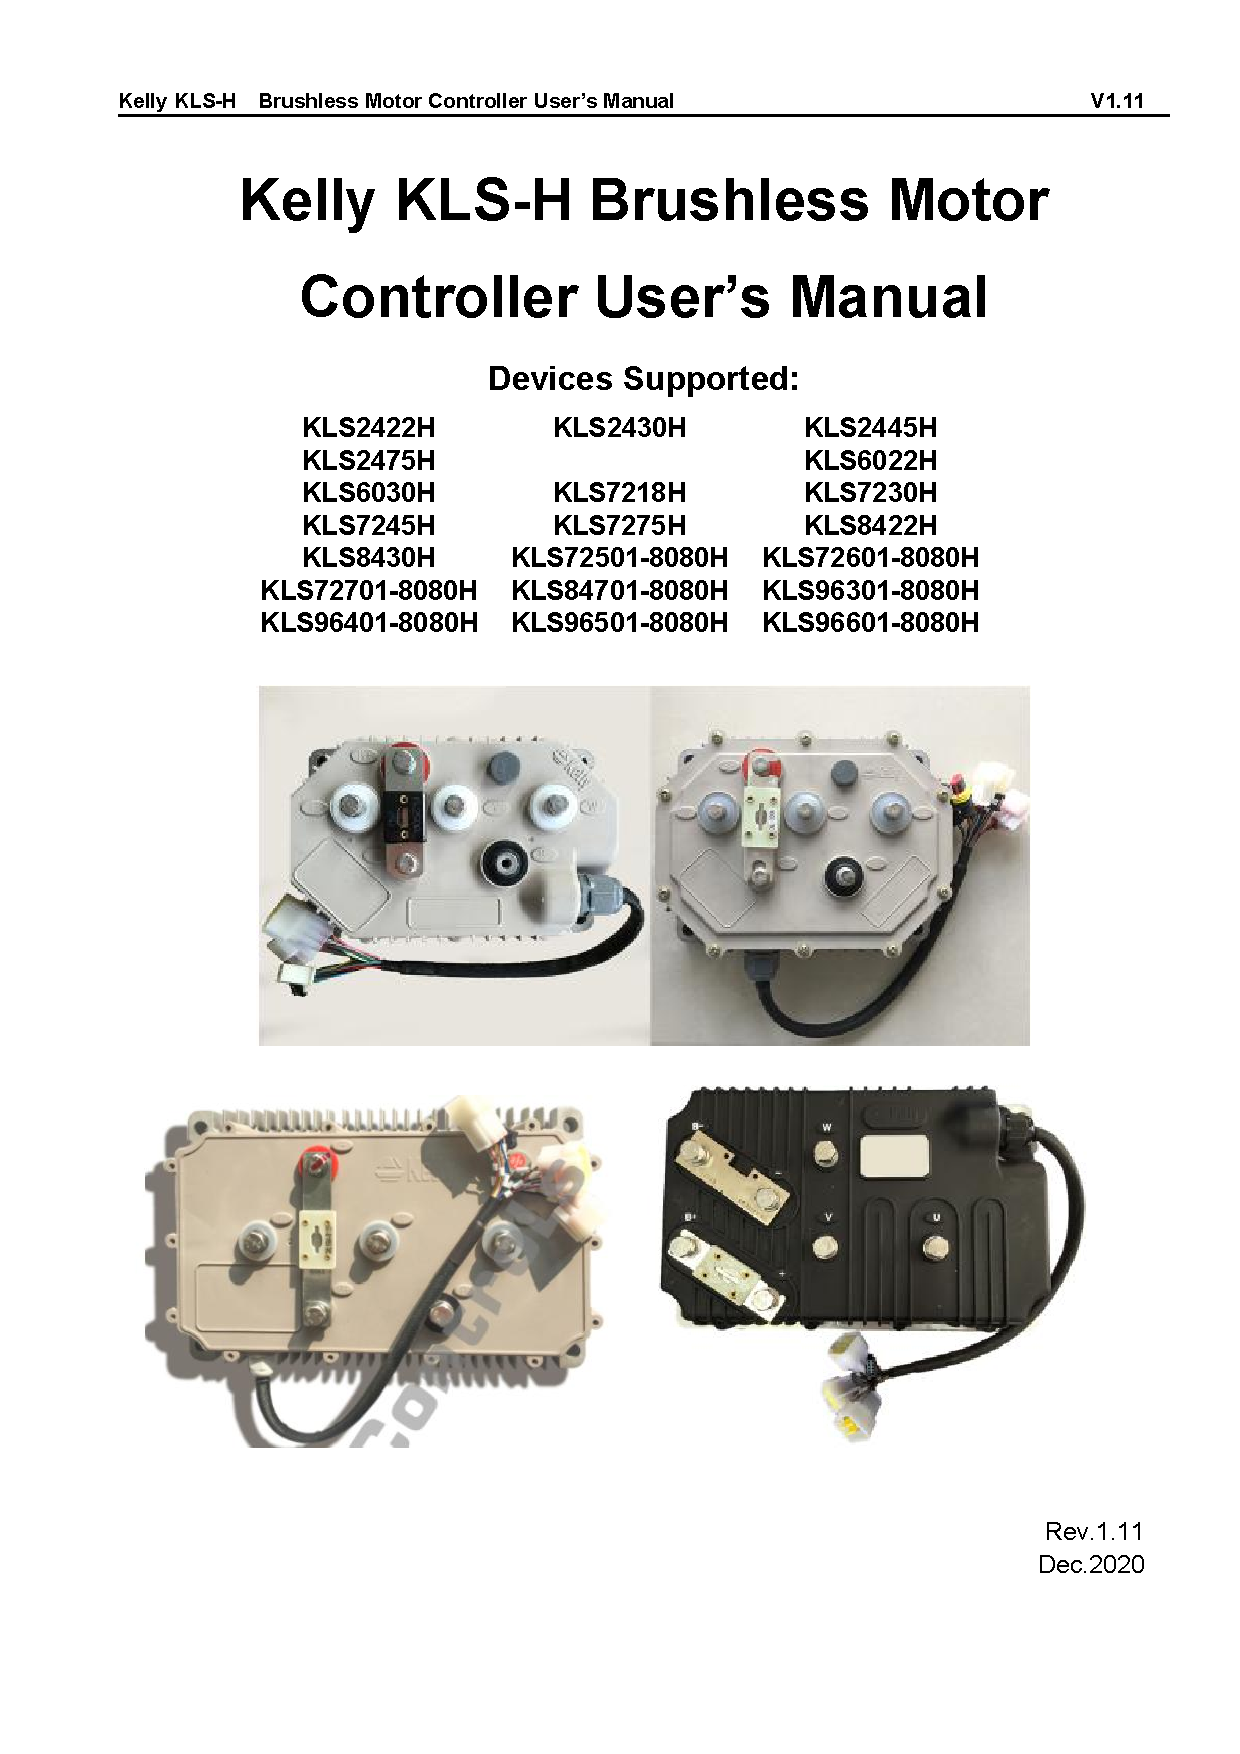
\includepdf[pages={1,4,5,6,7,10,12,13,14}]{dokumenti/KellyKLS}



%\chapter{JKH Foot Throttle}\label{gas}

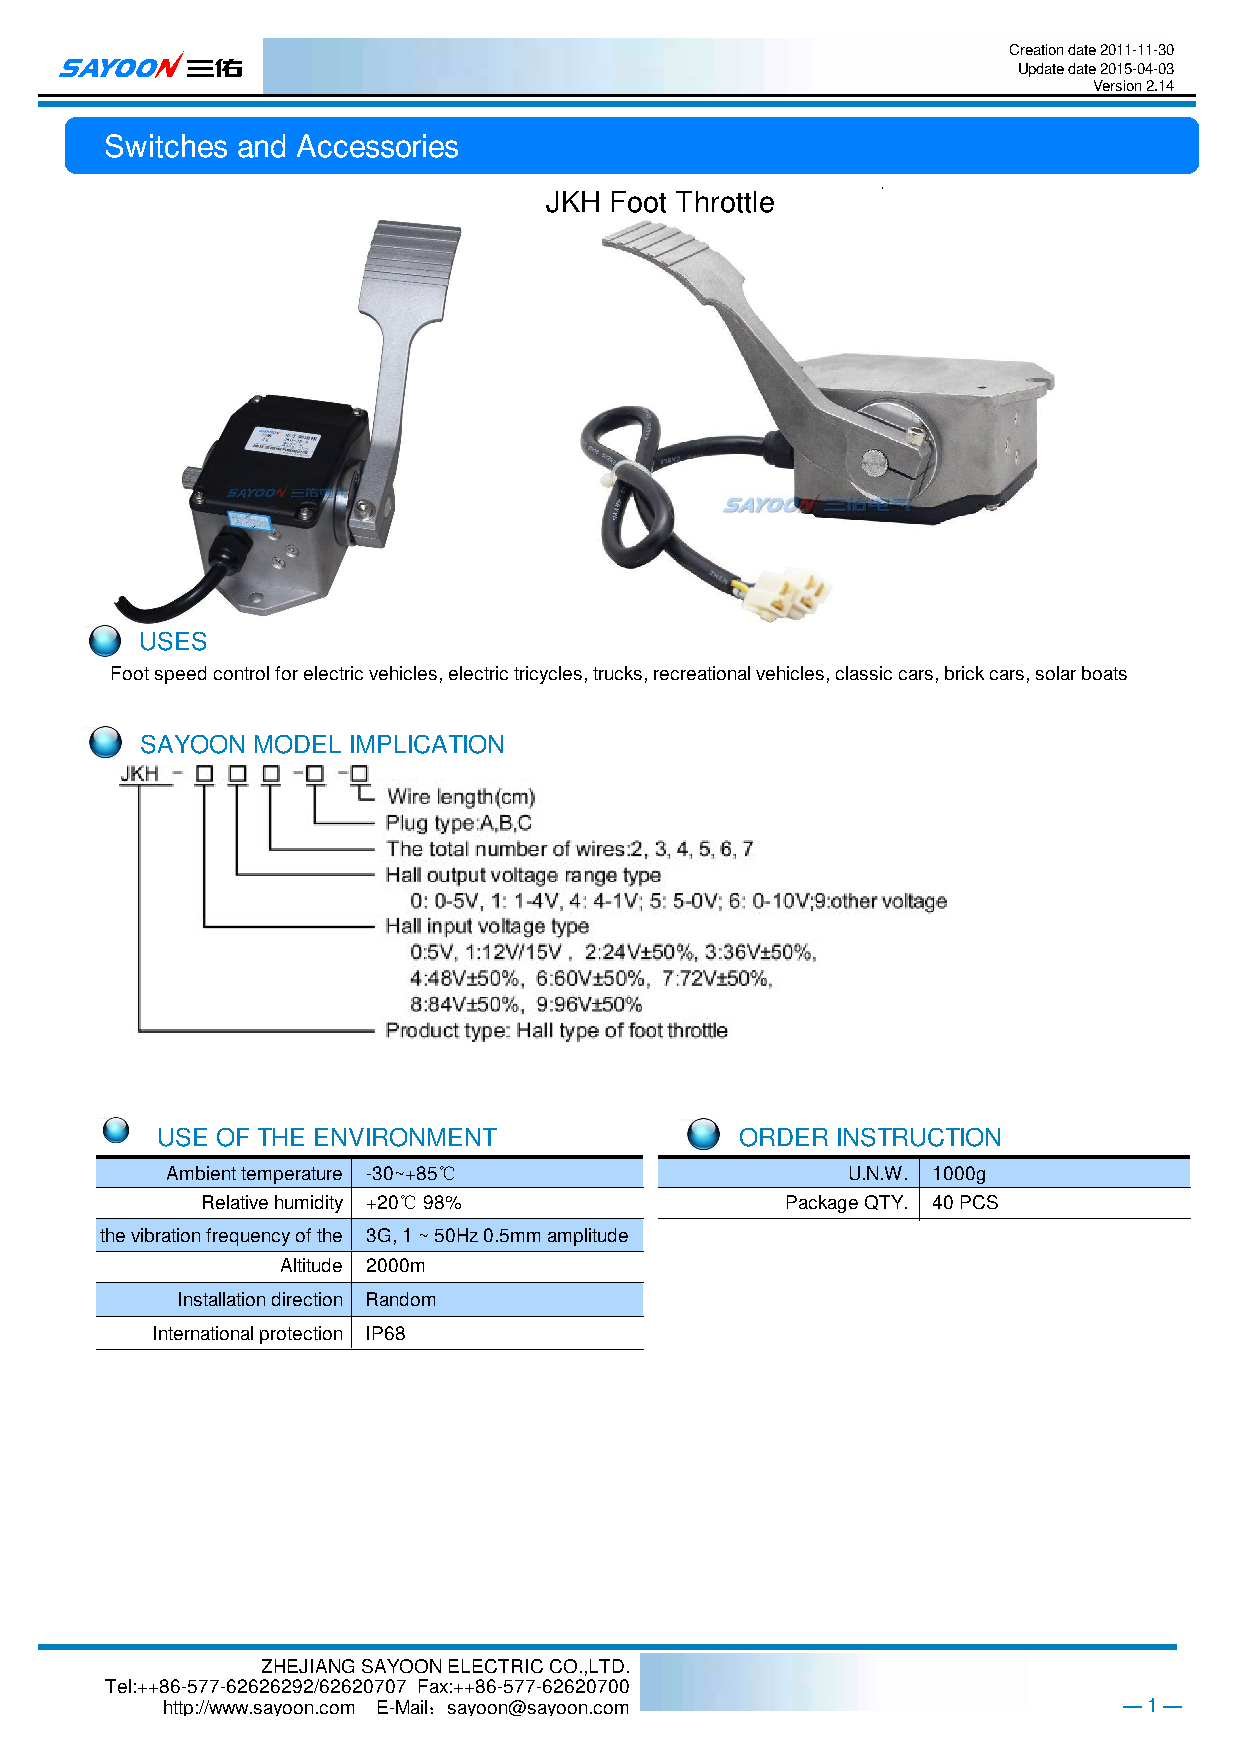
\includepdf[pages={1,2,3}]{dokumenti/foot_throttle}



\chapter{Control Box}\label{control}

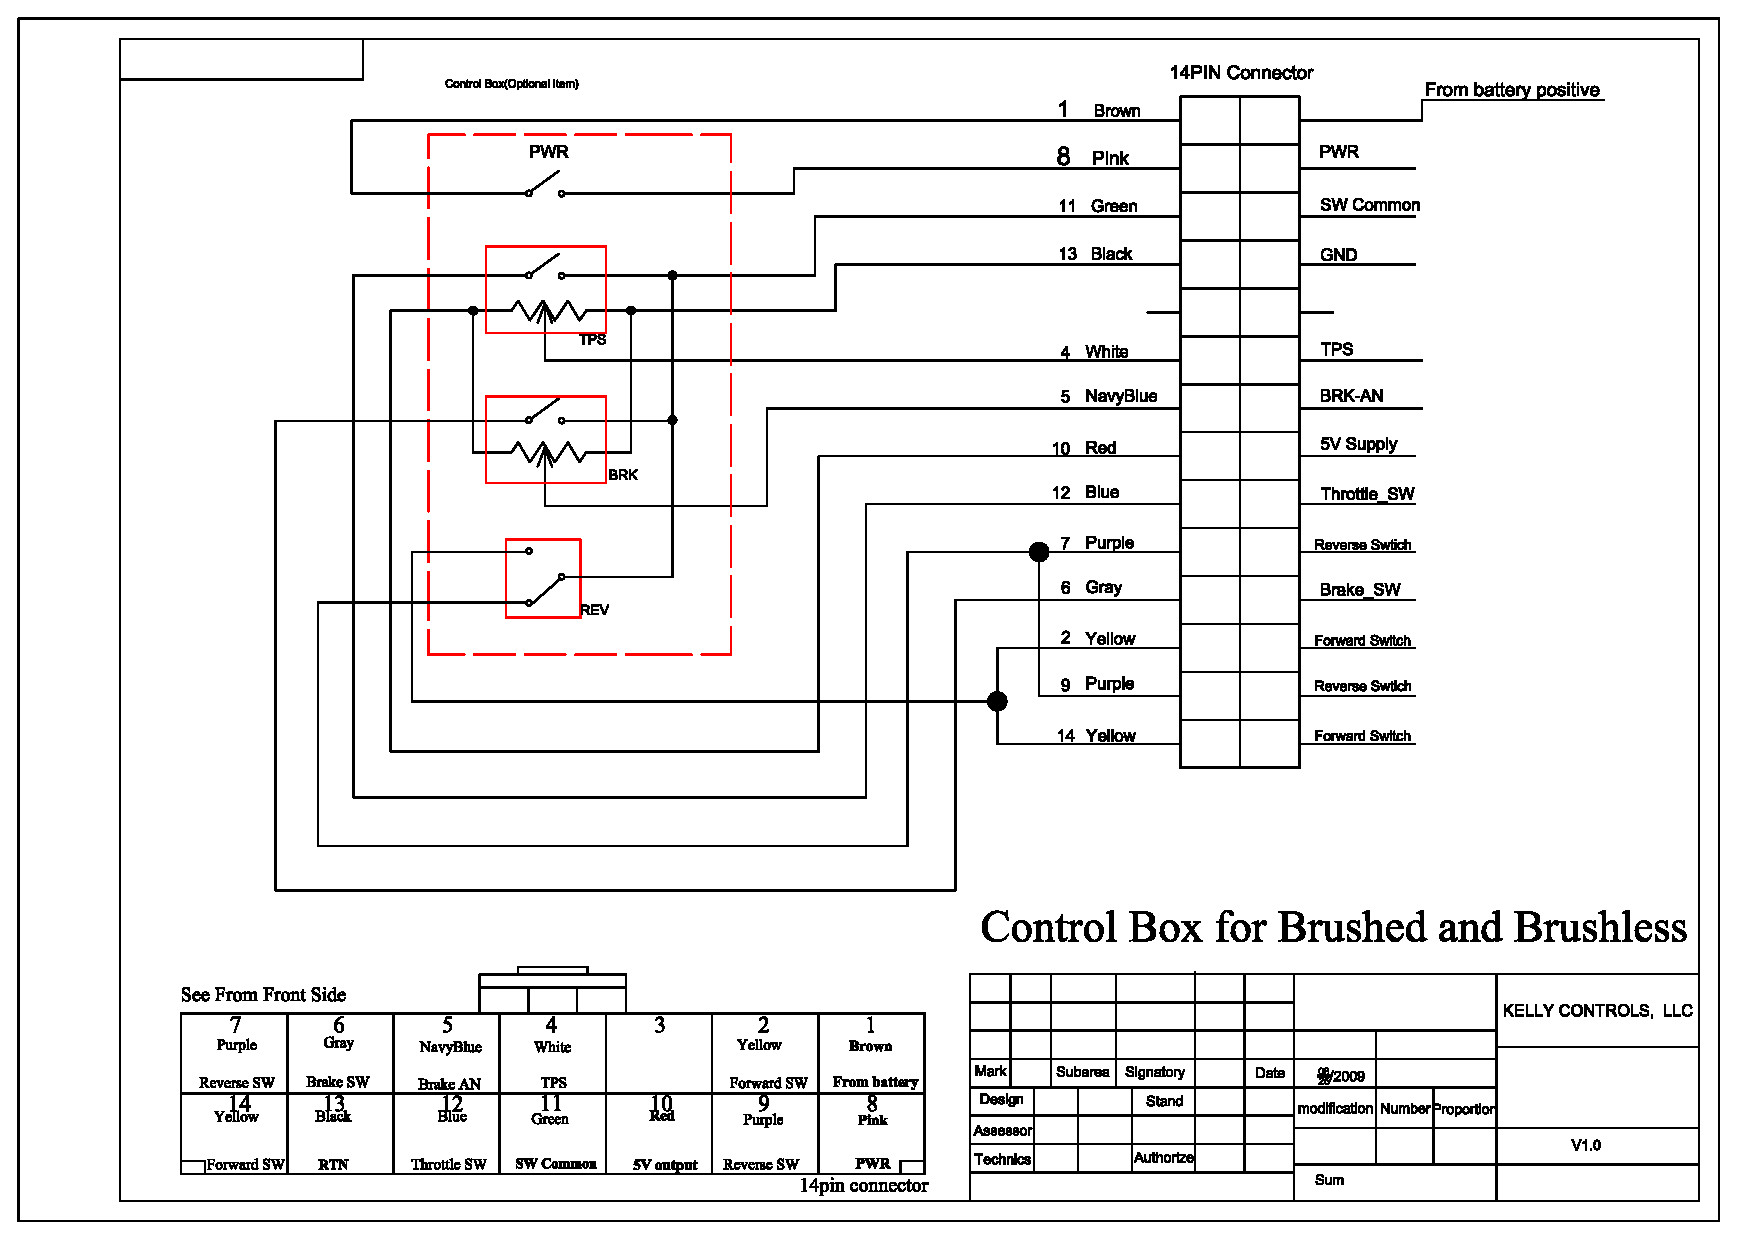
\includepdf[pages={-},angle=-90]{dokumenti/ControlBox}




\end{appendices}


%%%%%%%%%%%%%%%%%%%%%%%%%%%%%%%%%%%%%%%%%%%%%%%%%%%%%%%%%%%%%%%%%%%%
%\backmatter
%%%%%%%%%%%%%%%%%%%% LISTA PUBLIKACIJA %%%%%%%%%%%%%%%%%%%%%%%%%%%%%
%\chapter*{Lista publikacija}
%\addcontentsline{toc}{chapter}{Lista publikacija}

%%%%%%%%%%%%%%%%%%%%%%% LITERATURA %%%%%%%%%%%%%%%%%%%%%%%%%%%%%%%%%
\addcontentsline{toc}{chapter}{Literatura}
\bibliographystyle{IEEEtranETF} 
\bibliography{literatura}

%%%%%%%%%%%%%%%%%%%%%%%%%%% INDEKS POJMOVA %%%%%%%%%%%%%%%%%%%%%%%%%
%\addcontentsline{toc}{chapter}{Indeks pojmova}
%\printindex 


\end{document}
